\documentclass{article}

\usepackage{microtype}
\usepackage{graphicx}
\usepackage{subcaption}
\usepackage{booktabs}
\usepackage{hyperref}
\newcommand{\theHalgorithm}{\arabic{algorithm}}
\usepackage{icml2026}
\usepackage{amsmath}
\usepackage{amssymb}
\usepackage{mathtools}
\usepackage{amsthm}
\usepackage[capitalize,noabbrev]{cleveref}

\theoremstyle{plain}
\newtheorem{theorem}{Theorem}[section]
\newtheorem{proposition}[theorem]{Proposition}
\newtheorem{lemma}[theorem]{Lemma}
\newtheorem{corollary}[theorem]{Corollary}
\theoremstyle{remark}
\newtheorem{remark}[theorem]{Remark}

\newcommand{\simplex}{\Delta^{K-1}}
\newcommand{\R}{\mathbb{R}}
\renewcommand{\Pr}{\mathbb{P}}
\newcommand{\E}{\mathbb{E}}
\newcommand{\clr}{\mathrm{clr}}
\DeclareMathOperator{\expit}{expit}
\DeclareMathOperator{\logit}{logit}
\graphicspath{{figures/}}

\icmltitlerunning{Evaluating Conformal Prediction Regions for Compositional Outputs}

\begin{document}

\twocolumn[
  \icmltitle{Beyond Marginal Coverage: Evaluating Conformal Prediction\\
  Regions for Compositional (Sum-to-One) Outputs}

  \icmlsetsymbol{equal}{*}
  \begin{icmlauthorlist}
    \icmlauthor{Anonymous Authors}{anon}
  \end{icmlauthorlist}
  \icmlaffiliation{anon}{Anonymous Institution}
  \icmlcorrespondingauthor{Anonymous Authors}{anonymous@example.org}
  \icmlkeywords{conformal prediction, compositional data, uncertainty quantification}
  \vskip 0.3in
]

\printAffiliationsAndNotice{}

\begin{abstract}
Predictors whose output is a composition (a non-negative vector summing to one: softmax probabilities, topic or vote shares) are increasingly paired with conformal prediction regions in the simplex, but there is no shared recipe for judging whether such regions are \emph{reliable}. We study this evaluation question with a controlled comparison of split conformal regions built from eight nonconformity scores (Euclidean, total variation, sup-norm, Hellinger, KL, Aitchison log-ratio, a Mahalanobis log-ratio score, a normalised Euclidean score), two Mondrian variants and cross-conformal calibration, on 36 synthetic settings (logistic-normal, Dirichlet and multinomial targets, $K\in\{3,5,10\}$, 200 replicates each) and on human label distributions for CIFAR-10 test images (CIFAR-10H). We find that (i) marginal coverage is uninformative: all scores are valid (mean coverage 0.895--0.911), and a single-run coverage check cannot resolve $\pm0.02$ unless the calibration set has about $2000$ points, as the (known) Beta--Binomial law of one-run coverage, which we verify, predicts; (ii) region size depends strongly on the score's geometry and the noise family, with the Aitchison score giving regions $0.16$--$0.87\times$ the Euclidean size for strictly positive logistic-normal targets but $1.8$--$3.9\times$ for Dirichlet and multinomial targets with (near-)zeros; (iii) conditional coverage fails in score-specific ways: in closed form for $K{=}2$ the Euclidean score covers $0.83$ to $0.997$ of the targets at nominal $0.90$, and on CIFAR-10H the Euclidean regions cover $0.99$ and $0.72$ of the lowest- and highest-entropy predictions, repaired by Mondrian calibration at $+23\%$ size; (iv) log-ratio scores depend on the zero-replacement constant $\varepsilon$: we prove that the threshold grows as $\sqrt{g/K}\,\log(1/\varepsilon)$ once about an $\alpha$ fraction of calibration compositions contain a zero, and confirm the slope to within $2\%$. We state the conditions under which these conclusions hold and where they should not be extrapolated.
\end{abstract}

\section{Introduction}
\label{sec:intro}
Many predictors output a composition $f(x)\in\simplex=\{p\in\R^K_{\ge0}:\sum_k p_k=1\}$: the softmax of a classifier, a topic mixture, a market share. Users need to know whether a stated uncertainty is trustworthy. Conformal prediction \citep{vovk2005,lei2018,angelopoulos2021gentle} turns any score of disagreement $s(y,f(x))$ into a region $C(x)\subset\simplex$ with finite-sample marginal coverage under exchangeability, so the \emph{validity} question has a formal answer, whatever the score. What remains open for compositional outputs is practical: which geometry to use for the score (Euclidean, Hellinger, KL, log-ratio~\citep{aitchison1982}), how to handle exact zeros, which calibration scheme to use, and---the focus here---\emph{how to evaluate} such regions in a way that is informative rather than circular.

We ask four questions, formulated before running the main experiments: \textbf{RQ1} What can empirical marginal coverage tell us, and how much calibration/test data does a coverage check need? \textbf{RQ2} How do region sizes of different geometries compare, and does the answer depend on the noise family and on how ``size'' is measured? \textbf{RQ3} Where does conditional coverage fail, which scores or calibrations repair it, and at what cost? \textbf{RQ4} How do log-ratio scores behave when targets contain exact zeros? Our a-priori expectations were: marginal coverage does not discriminate (H1); the best geometry follows the noise geometry (H2); the ranking of scores changes with the size measure (H3); log-ratio scores are fragile with zeros (H4). H1, H2, H4 are supported; H3 is only partly supported (Sec.~\ref{sec:res-size}).

\textbf{Contributions.} (1) An evaluation protocol for simplex-valued conformal regions combining the exact coverage law of a single run, group-conditional coverage gaps, size under two reference measures, and sensitivity to the zero-replacement constant. (2) Three propositions with derivations and numerical checks: the Beta--Binomial law of one-run coverage (a consequence of known results~\citep{vovk2012conditional}, used here as an evaluation tool); a pivotality condition for conditional coverage with a closed form for $K{=}2$; and an exact asymptotic law for the log-ratio threshold under zero replacement. (3) A reproducible empirical study (36 synthetic cells $\times$ 200 replicates, plus CIFAR-10H) with uncertainty quantification. (4) Explicit conditions of validity and non-extrapolation (Sec.~\ref{sec:disc}).

\section{Related Work}
\label{sec:related}
\textbf{Conformal prediction.} Split/inductive conformal prediction \citep{papadopoulos2002,vovk2005,lei2018} gives marginal coverage for any score; its coverage given the calibration set is Beta distributed \citep{vovk2012conditional}, which we use as an evaluation tool. Jackknife+ and cross-conformal calibration \citep{barber2021jackknife,vovk2015cross} reuse data at the price of a weaker ($1-2\alpha$) guarantee; we test it at equal labelled budget. Exact conditional coverage is impossible in a distribution-free sense \citep{vovk2012conditional,barber2021limits}; relaxations include Mondrian/class-conditional calibration \citep{vovk2005,ding2023clustered}, multivalid methods \citep{jung2022batch} and conditional guarantees over function classes \citep{gibbs2023conditional}. Coverage under covariate shift \citep{tibshirani2019} is outside our scope.

\textbf{Probability-vector outputs.} For classifiers, conformal methods build label sets from softmax scores \citep{romano2020aps,angelopoulos2020raps}; \citet{javanmardi2024credal} predict credal sets (sets of distributions), and \citet{cresswell2024disparate} study the downstream effect of prediction sets on decisions. Multi-target conformal regions in $\R^d$ use box, ellipsoid or copula-based scores \citep{messoudi2021copula}. We instead study regions \emph{in the simplex} for a compositional target, and compare geometries that respect (Aitchison) or ignore (Euclidean) the simplex constraint.

\textbf{Compositional data analysis.} Aitchison geometry, the centred and isometric log-ratio transforms and the logistic-normal family \citep{aitchison1982,aitchison1980,egozcue2003} are the standard tools; their known difficulty with exact zeros motivates our fourth question. We do not claim a new method: our contribution is the evaluation analysis, its theory, and the empirical map of when each choice works.

\section{Setting, Methods and Evaluation Protocol}
\label{sec:method}
\textbf{Setting.} Data $(X,Y)$ with $Y\in\simplex$; a predictor $f:\mathcal X\to\mathrm{int}\,\simplex$ trained on separate data; $n$ calibration pairs exchangeable with the test pair. A score $s(y,p)\ge0$ defines the region $C(x)=\{y\in\simplex: s(y,f(x))\le\hat q\}$ with $\hat q$ the $\lceil(n+1)(1-\alpha)\rceil$-th smallest calibration score ($\infty$ if it exceeds $n$); $\alpha=0.1$ throughout.

\textbf{Scores} (all computed with a closed-form membership test, so regions need not be parametrised): Euclidean $\ell_2=\|y-p\|_2$; total variation $\tfrac12\|y-p\|_1$; $\ell_\infty$; Hellinger $\|\sqrt y-\sqrt p\|_2$; $\mathrm{KL}(y\|p)$; Aitchison $\|\clr(y_\varepsilon)-\clr(p)\|_2$ with $y_\varepsilon=(y+\varepsilon\mathbf 1)/(1+K\varepsilon)$ (additive zero replacement, $\varepsilon=10^{-3}$ synthetic, $10^{-2}\approx$ half a vote for CIFAR-10H); a Mahalanobis score on $\mathrm{ilr}(y_\varepsilon)-\mathrm{ilr}(p)$ with a residual covariance estimated on an auxiliary fold; and $\ell_2/\hat\sigma(p)$ where $\hat\sigma$ is a linear function of the Gini impurity $1-\|p\|^2$ fitted on the auxiliary fold. Validity never depends on the auxiliary fold.

\textbf{Calibration schemes.} (a) Split conformal. (b) Mondrian: separate $\hat q$ in three terciles of the entropy of $f(x)$ (cut points from the auxiliary fold). (c) Five-fold cross-conformal \citep{vovk2015cross} generalised to arbitrary scores: $y\in C(x)$ iff $\#\{i: s(y,f_{-k(i)}(x))>R_i\}<(1-\alpha)(N+1)$, with $R_i$ the out-of-fold scores.

\textbf{Evaluation protocol.} For each replicate we report: \emph{marginal coverage} on a test set; \emph{group-conditional coverage}, pooled over replicates, in entropy terciles of $f(x)$ and in argmax-class groups, summarised by the \emph{gap} = worst group $|\text{coverage}-(1-\alpha)|$ (ent.-gap, arg-gap; their noise floor is about $0.003$--$0.008$); and \emph{size} = $\E_{x}\,\mu(C(x))$ for two reference measures $\mu$: the empirical marginal law of $Y$ (\emph{pool size}, from an independent pool of 1000 targets) and the uniform (Dirichlet(1)) measure on the simplex (\emph{uniform size}, 4000 draws, $K\le5$). Uncertainty: $R$ independent replicates (new world, data, splits), mean $\pm$ 95\% normal CI over replicates, paired differences within replicate with Holm correction over all 252 size comparisons; group gaps have bootstrap CIs over replicates.

\section{Theory}
\label{sec:theory}
Proofs are in Appendix~\ref{app:proofs}; all three statements are checked numerically in Sec.~\ref{sec:results}.

\begin{proposition}[One-run coverage law]\label{prop:beta}
Let $f$ be fixed and the scores $S_1,\dots,S_{n+1}$ i.i.d.\ with continuous cdf $F$. With $k=\lceil(n+1)(1-\alpha)\rceil$, $l=n+1-k=\lfloor(n+1)\alpha\rfloor$, the coverage given the calibration set is $C_{\rm cal}=F(\hat q)\sim\mathrm{Beta}(k,l)$, with mean $k/(n+1)\ge1-\alpha$ and variance $kl/((n+1)^2(n+2))\approx\alpha(1-\alpha)/(n+2)$. The number of covered points among $m$ test points is $\mathrm{BetaBin}(m;k,l)$, so the empirical coverage has variance $\approx\alpha(1-\alpha)\,(\tfrac1{n+2}+\tfrac1m)$.
\end{proposition}
\emph{Consequence.} A one-run check ``$|\widehat{\rm cov}-0.9|\le\delta$'' of a valid method fails with a probability computable from this law, \emph{whatever the score}. For $\delta=0.02$, $n=500$ and $m=10^4$ the false-alarm probability is $14\%$; it falls to $0.6\%$ only at $n=2000$, and is $50\%$ or more at $n=100$ for every $m$ (Fig.~\ref{fig:theory}b).

\begin{proposition}[Pivotal scores and conditional coverage]\label{prop:pivot}
(a) If $S=s(Y,f(X))$ is independent of $X$, then for every calibration set and every $x$, $\Pr(Y\in C(X)\mid X=x,D_{\rm cal})=F(\hat q)$: conditional coverage is constant in $x$. (b) For the logistic-normal model $Y=\mathrm{softmax}(\eta(X)+\sigma\xi)$, $\xi\sim N(0,I_K)$, and $f=\mathrm{softmax}(\eta)$, the Aitchison score ($\varepsilon=0$) equals $\sigma\|\xi-\bar\xi\mathbf 1\|\sim\sigma\chi_{K-1}$, hence is pivotal. (c) For $K=2$, put $u=\logit f_1$, $\tau=\sigma\sqrt2$, and let the $\ell_2$ region be $|y_1-f_1|\le r$. Then
\[
c(f_1)=\Phi\!\Big(\tfrac{\logit(f_1+r)-u}{\tau}\Big)-\Phi\!\Big(\tfrac{\logit(f_1-r)-u}{\tau}\Big),
\]
with $\logit(t)=\pm\infty$ for $t\ge1$, $t\le0$. $c$ is continuous with $c(f_1)\to1$ as $f_1\to0$ or $1$; since its average over $f_1(X)$ equals $1-\alpha$ for the population threshold, $c<1-\alpha$ on a set of positive probability: \emph{no Euclidean region can be conditionally valid under this noise}.
\end{proposition}

\begin{proposition}[Zero replacement and the log-ratio threshold]\label{prop:zero}
Let $y\in\simplex$ have exactly $z$ zero entries, $0<z<K$, $f\in\mathrm{int}\,\simplex$ fixed, $L=\log(1/\varepsilon)$. Then $d_A(y_\varepsilon,f)=L\sqrt{z(K-z)/K}+O(1)$ as $\varepsilon\to0$, while $d_A(y_\varepsilon,f)=O(1)$ if $z=0$. Hence for a fixed calibration set with $g_i=z_i(K-z_i)$,
\[
\lim_{\varepsilon\to0}\hat q/\log(1/\varepsilon)=\sqrt{g_{(k)}/K},
\]
where $g_{(k)}$ is the $k$-th smallest $g_i$. If $g_{(k)}>0$ (equivalently, at least $l\approx\alpha(n+1)$ calibration compositions contain a zero), then $\hat q\to\infty$ linearly in $\log(1/\varepsilon)$ and the uniform size of $C(x)$ tends to $1$; if $g_{(k)}=0$, $\hat q$ stays bounded.
\end{proposition}
The practical reading: the Aitchison score is safe as $\varepsilon$ varies only when fewer than about an $\alpha$ fraction of targets contain zeros; otherwise $\varepsilon$ is a hidden tuning parameter of the \emph{evaluation} (it controls region size) rather than a numerical detail.

\section{Experimental Setup}
\label{sec:setup}
\textbf{Synthetic data.} Features $x\sim N(0,I_5)$; $\eta(x)=W^\top x$ with $W_{jk}\sim N(0,0.6^2)$ redrawn per replicate; $m(x)=\mathrm{softmax}(\eta)$. Targets: \emph{LN-homo} $Y=\mathrm{softmax}(\eta+0.5\,\xi)$; \emph{LN-hetero} noise scale $0.35\,e^{0.5x_1}$; \emph{Dirichlet} $Y\sim\mathrm{Dir}(20\,m(x))$; \emph{Multinomial} $Y=\mathrm{Mult}(20,m(x))/20$ (exact zeros in 64\% of the $K{=}5$ targets). $K\in\{3,5,10\}$, $n_{\rm cal}\in\{50,200,1000\}$, 200 replicates per cell (7200 runs). The predictor is a multinomial-logit regression with soft labels (cross-entropy, ridge $10^{-3}$) fit on 1000 points; 500 auxiliary, 1000 test and 1000 pool points are independent. Extra runs vary the predictor sample size ($n_{\rm train}\in\{30,\dots,3000\}$), the zero constant $\varepsilon$, and the calibration scheme (equal labelled budget $N\in\{60,150,400\}$; 100 replicates).

\textbf{Real data.} CIFAR-10H \citep{peterson2019cifar10h}: for the 10000 CIFAR-10 \citep{krizhevsky2009} test images, the proportions of $\approx$50 human annotators choosing each class ($K=10$; 44\% unanimous; 99.97\% of vectors contain at least one zero, 8.1 zero entries on average). The predictor is a publicly available ResNet-20 trained on the CIFAR-10 training set only \citep{chenyaofo2021cifar} (92.1\% test accuracy), used either as the raw softmax or after temperature scaling \citep{guo2017calibration} fit on the auxiliary fold. Each replicate draws random disjoint auxiliary (1000), calibration ($n\in\{100,500,2000\}$) and test (2000) subsets of the 10000 images; 100 replicates. Intervals therefore reflect split-to-split variability within a fixed finite pool, not sampling of new images.

\begin{figure*}[t]
\centering
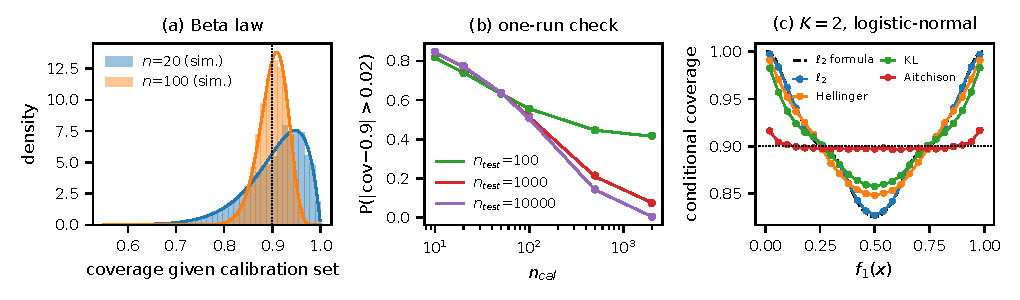
\includegraphics[width=\textwidth]{fig_theory.pdf}
\caption{Evaluation theory vs.\ simulation. (a) Coverage given the calibration set ($\ell_2$ score, logistic-normal, oracle $f$; $2\times10^4$ calibration draws per $n$) against the Beta law. (b) Probability that a valid method's one-run coverage lies more than $0.02$ from $0.9$; lines: Beta--Binomial law, dots: simulation. (c) $K{=}2$ conditional coverage vs.\ $f_1(x)$ ($\tau=1$, $n_{\rm cal}=2000$, 40 calibrations); dashed: closed form of Prop.~\ref{prop:pivot}c.}
\label{fig:theory}
\end{figure*}

\section{Results}
\label{sec:results}
\subsection{Marginal coverage is valid and uninformative (RQ1)}
Across all 36 cells, every non-Mondrian score has mean coverage between $0.895$ and $0.911$ (Table~\ref{tab:validity}, App.~\ref{app:tables}); the deviation from the exact expectation $k/(n+1)$ has $|z|\le2.96$ for seven scores, and $3.41$ for one of $288$ score-cell pairs for Aitchison (Bonferroni threshold $\approx3.8$), so no evidence against validity. The Beta law of Prop.~\ref{prop:beta} matches simulation closely (Fig.~\ref{fig:theory}a, Table~\ref{tab:beta}): means within $1.5\times10^{-3}$, standard deviations within $1.3\%$, KS statistics $\le0.013$ for $2\times10^4$ draws, for the $\ell_2$, Aitchison and (multinomial) TV scores alike. Mondrian regions are valid but conservative in small groups (mean coverage $0.928$, $0.907$, $0.901$ at $n_{\rm cal}=50,200,1000$, as the rounding in $k$ predicts). \emph{Coverage therefore cannot discriminate between scores, and a single coverage number is a noisy check}: the standard deviation of one-run coverage is $0.041$ at $n=50$ and $0.013$ at $n=500$ (Fig.~\ref{fig:theory}b).

\begin{table*}[t]
\caption{Synthetic results, $K=5$, $n_{\rm cal}=200$, 200 replicates. \emph{size}: mean pool size (fraction of reference targets inside the region; bold = smallest; 95\% CI half-widths 0.004--0.013), \emph{gap}: worst entropy-tercile coverage deviation $|{\rm cov}-0.9|$ (95\% bootstrap half-width $\le 0.006$). Coverage of every row is within $0.898$--$0.908$ (App.~\ref{app:tables}). $K{=}3,10$ and other $n_{\rm cal}$ in App.~\ref{app:tables}.}
\label{tab:main}
\centering\small
\begin{tabular}{lrrrrrrrr}
\toprule
 & \multicolumn{2}{c}{LN-homo} & \multicolumn{2}{c}{LN-hetero} & \multicolumn{2}{c}{Dirichlet} & \multicolumn{2}{c}{Multinom.} \\
Score & size & gap & size & gap & size & gap & size & gap \\
\midrule
$\ell_2$ & 0.149 & 0.026 & 0.125 & 0.020 & 0.108 & 0.037 & 0.114 & 0.042 \\
TV & 0.128 & 0.043 & 0.109 & 0.024 & 0.103 & 0.055 & 0.111 & 0.055 \\
$\ell_\infty$ & 0.179 & 0.030 & 0.149 & 0.022 & 0.129 & 0.035 & 0.132 & 0.035 \\
Hellinger & 0.088 & 0.042 & 0.082 & 0.016 & 0.084 & 0.030 & 0.144 & 0.021 \\
KL & 0.088 & 0.041 & 0.080 & 0.016 & \textbf{0.084} & 0.024 & \textbf{0.101} & 0.028 \\
Aitchison & \textbf{0.067} & 0.003 & \textbf{0.076} & 0.030 & 0.272 & 0.086 & 0.443 & 0.018 \\
Mahal.-ilr & 0.067 & 0.004 & 0.077 & 0.031 & 0.280 & 0.090 & 0.452 & 0.016 \\
$\ell_2/\hat\sigma$ & 0.160 & 0.040 & 0.133 & 0.034 & 0.115 & 0.024 & 0.120 & 0.021 \\
$\ell_2$-Mond. & 0.158 & 0.008 & 0.136 & 0.007 & 0.116 & 0.008 & 0.121 & 0.006 \\
Ait.-Mond. & 0.071 & 0.007 & 0.081 & 0.010 & 0.241 & 0.007 & 0.451 & 0.013 \\
\bottomrule
\end{tabular}
\end{table*}

\subsection{Region size depends on geometry, noise family and measure (RQ2)}
\label{sec:res-size}
Table~\ref{tab:main} and Fig.~\ref{fig:relsize} show that no score dominates. For strictly positive logistic-normal targets the log-ratio scores give the smallest regions, and the advantage grows with $K$: Aitchison regions have $0.79$, $0.45$, $0.16\times$ the $\ell_2$ pool size at $K=3,5,10$ (LN-homo, $n_{\rm cal}=200$) and $0.87,0.61,0.35\times$ for heteroscedastic noise. For Dirichlet and multinomial targets the picture reverses: Aitchison is $1.8$--$2.5\times$ larger than $\ell_2$ (Dirichlet) and $2.8$--$3.9\times$ (multinomial), all Holm-significant. Hellinger is smaller than $\ell_2$ in 27 cells (all LN, LN-hetero, Dirichlet cells) but larger in the 9 multinomial cells; KL is the best or tied-best non-log-ratio score in the Dirichlet and multinomial settings (KL vs.\ Hellinger: 24 of 36 cells smaller, 4 larger, 8 n.s.). The crude normalised score $\ell_2/\hat\sigma$ never helps: it is larger than $\ell_2$ in 24 cells ($+4$--$6\%$) and indistinguishable in 12. With a weaker or stronger predictor ($n_{\rm train}\in[30,3000]$, $K{=}5$) the winners are unchanged: Aitchison for both LN families, KL or Hellinger (near-tied) for Dirichlet and KL for multinomial targets (App.~\ref{app:tables}).

\begin{figure*}[t]
\centering
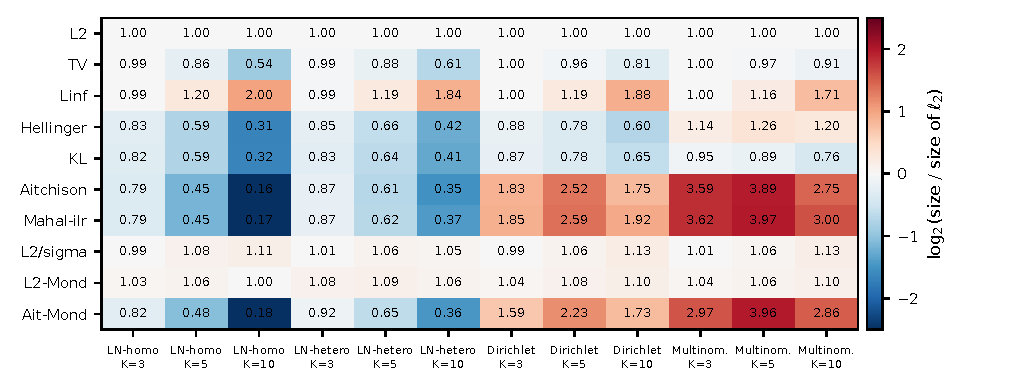
\includegraphics[width=0.85\textwidth]{fig_relsize.pdf}
\caption{Pool size relative to $\ell_2$ ($n_{\rm cal}=200$; entries are ratios; blue: smaller than $\ell_2$, red: larger).}
\label{fig:relsize}
\end{figure*}

\textbf{Does the size measure matter?} We expected the ranking to depend on the reference measure (H3). Over the 24 cells with $K\le5$, pool and uniform sizes give Kendall $\tau$ between methods with median $0.93$ (min $0.64$), so the overall ranking is largely stable; but the \emph{best} method differs in $11/24$ cells, always among near-ties (e.g.\ Aitchison vs.\ KL in LN-homo, $K{=}3$: pool sizes $0.79$ and $0.82$ of $\ell_2$; Table~\ref{tab:measure}, App.). Hence ``which of two close scores is smaller'' should not be reported under a single measure; the large effects above (factors 1.5--4) are measure-robust.

\begin{figure*}[t]
\centering
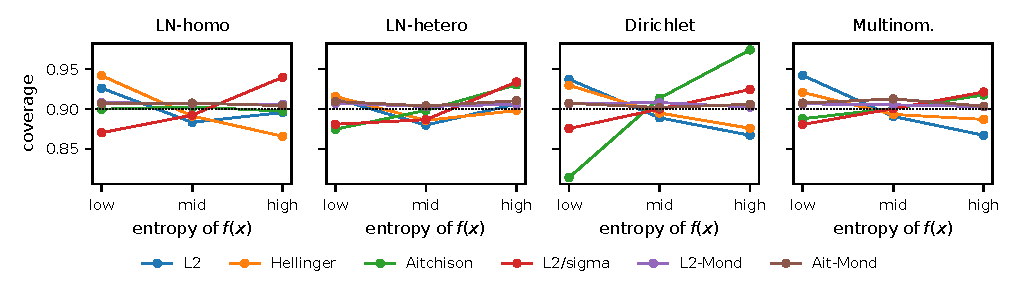
\includegraphics[width=\textwidth]{fig_cond_entropy.pdf}
\caption{Conditional coverage by entropy tercile of $f(x)$ ($K=5$, $n_{\rm cal}=200$, pooled over 200 replicates; dotted: $0.9$). All curves have marginal coverage $\approx0.9$.}
\label{fig:cond}
\end{figure*}

\subsection{Conditional coverage fails in score-specific ways (RQ3)}
All scores share marginal coverage $\approx0.9$ but differ in coverage across predicted-entropy terciles (Fig.~\ref{fig:cond}, gap columns of Table~\ref{tab:main}). In the logistic-normal model the Aitchison score is near-pivotal (Prop.~\ref{prop:pivot}b is exact for the oracle centre $f=\mathrm{softmax}(\eta)$; here $f$ is the fitted regression): gap $0.003$ (CI $0.002$--$0.007$) versus $0.026$ for $\ell_2$ and $0.042$ for Hellinger. This advantage is specific to the noise family: for Dirichlet targets the Aitchison gap is the \emph{worst} ($0.086$ vs.\ $0.037$), and with heteroscedastic noise it is $0.030$. The $K{=}2$ closed form of Prop.~\ref{prop:pivot}c is confirmed (Fig.~\ref{fig:theory}c): the Euclidean score covers $0.827$ at $f_1=0.5$ and $0.997$ near the boundary, the closed form deviating from simulation by at most $0.002$, while Aitchison is flat ($0.897$--$0.900$ for $0.1<f_1<0.9$; it rises to $0.917$ at $f_1=0.02$ because the replacement $\varepsilon=10^{-3}$ breaks pivotality). The worst coverage of the closed form is $0.80$, $0.83$, $0.88$ for $\tau=0.5,1,1.5$ (App.).

Mondrian calibration on entropy terciles removes the entropy gap for both scores (gap $0.006$--$0.013$, about the rounding floor), but it is not free: for $\ell_2$ it enlarges regions by $47\%$, $6\%$, $0.5\%$ at $n_{\rm cal}=50,200,1000$ (averages over cells), and since the grouping is on the same variable on which we measure the gap this favours Mondrian; it does not repair other groupings: at $K=10$ the argmax-class gap of $\ell_2$ and $\ell_2$-Mondrian are both $0.087$ (LN-homo) whereas Aitchison reaches $0.014$ in that setting.

\begin{figure*}[t]
\centering
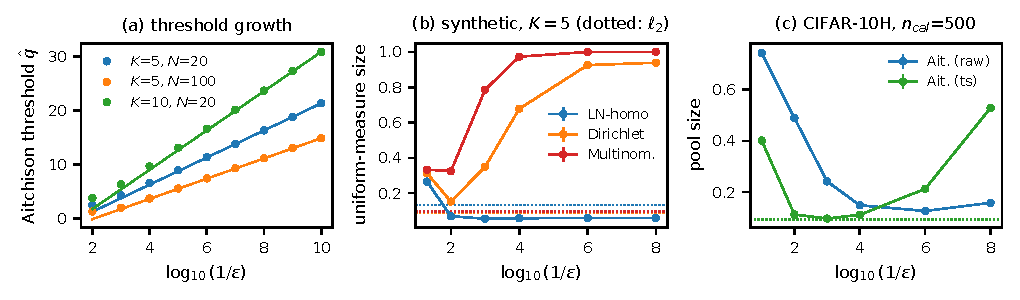
\includegraphics[width=\textwidth]{fig_zero.pdf}
\caption{Zero-replacement sensitivity of the Aitchison score. (a) Mean threshold $\hat q$ vs.\ $\log_{10}(1/\varepsilon)$ for multinomial targets (200 replicates); lines: slope $\sqrt{g_{(k)}/K}$ of Prop.~\ref{prop:zero}, anchored at the smallest $\varepsilon$. (b) Uniform-measure size, $K{=}5$, $n_{\rm cal}=200$ (dotted: $\ell_2$). (c) CIFAR-10H pool size ($n_{\rm cal}=500$; dotted: $\ell_2$).}
\label{fig:zero}
\end{figure*}

\subsection{Zeros make the log-ratio score hostage to $\varepsilon$ (RQ4)}
The slope of $\hat q$ against $\log(1/\varepsilon)$ measured between $\varepsilon=10^{-8}$ and $10^{-10}$ agrees with Prop.~\ref{prop:zero} to within $1.6\%$ (range $0.05$--$1.6\%$) in all six $(K,N)$ settings (mean over 200 replicates; e.g.\ $K=5,N=20$: $1.088\pm0.004$ vs.\ $1.090$; $K=10,N=20$: $1.555\pm0.001$ vs.\ $1.580$; Table~\ref{tab:zero}, App.). Both regimes of the proposition occur: for $K{=}3,N{=}100$, only 8\% of targets contain a zero ($<\alpha$) and 65\% of replicates have $g_{(k)}=0$ with a bounded threshold. In the size experiments the multinomial uniform size reaches $1.000$ for $\varepsilon\le10^{-6}$ and Dirichlet $0.94$ at $10^{-8}$, while for logistic-normal targets (no zeros) the size is flat for $\varepsilon\le10^{-4}$. The size is non-monotone in $\varepsilon$ (large $\varepsilon$ distorts the data), and the best $\varepsilon$ on our grid depends on the noise family ($10^{-3}$ for LN, $10^{-2}$ for Dirichlet/multinomial). Even at its best grid value the Aitchison pool size is $0.138$ (Dirichlet) and $0.244$ (multinomial) vs.\ $0.084$ (KL) and $0.101$ (KL) (K=5, $n_{\rm cal}=200$); the $\varepsilon$ choice is moreover made with knowledge of region size, i.e.\ optimistic.

\subsection{Calibration scheme and predictor quality}
At equal labelled budget, five-fold cross-conformal regions are smaller than split regions by $15\%$, $9\%$, $1\%$ for $N=60,150,400$ (mean over 4 noise families $\times$ $\ell_2$/Hellinger/Aitchison; 12 cells each; Table~\ref{tab:cv}, App.), with coverage $0.899$--$0.918$ (the theoretical guarantee is $1-2\alpha$; we do not observe violations, but we test only $K=5$ and three scores). The gain is concentrated at $N\lesssim150$.

\subsection{Real data: CIFAR-10H}
\begin{table*}[t]
\caption{CIFAR-10H, $n_{\rm cal}=500$, 100 replicates. cov.: marginal coverage; size: pool size (bold: smallest); ent.-gap and arg-gap: worst entropy-tercile / argmax-class deviation from $0.9$. 95\% CI half-widths: coverage $\le0.003$, size $\le 0.006$, ent.-gap and arg-gap $\le0.008$.}
\label{tab:cifar}
\centering\small
\begin{tabular}{lrrrrrrrr}
\toprule
 & \multicolumn{4}{c}{raw softmax} & \multicolumn{4}{c}{temperature-scaled} \\
Score & cov. & size & ent.-gap & arg-gap & cov. & size & ent.-gap & arg-gap \\
\midrule
$\ell_2$ & 0.897 & 0.094 & 0.182 & 0.092 & 0.899 & 0.094 & 0.182 & 0.074 \\
TV & 0.897 & 0.095 & 0.182 & 0.094 & 0.898 & 0.094 & 0.187 & 0.079 \\
$\ell_\infty$ & 0.897 & 0.095 & 0.180 & 0.092 & 0.898 & 0.094 & 0.186 & 0.075 \\
Hellinger & 0.898 & \textbf{0.094} & 0.176 & 0.089 & 0.897 & 0.092 & 0.191 & 0.082 \\
KL & 0.898 & 0.095 & 0.108 & 0.134 & 0.898 & \textbf{0.092} & 0.160 & 0.078 \\
Aitchison & 0.903 & 0.489 & 0.176 & 0.092 & 0.902 & 0.113 & 0.085 & 0.092 \\
Mahal.-ilr & 0.904 & 0.484 & 0.177 & 0.036 & 0.901 & 0.106 & 0.079 & 0.053 \\
$\ell_2/\hat\sigma$ & 0.899 & 0.134 & 0.092 & 0.126 & 0.900 & 0.131 & 0.019 & 0.152 \\
$\ell_2$-Mond. & 0.902 & 0.116 & 0.005 & 0.140 & 0.901 & 0.105 & 0.005 & 0.136 \\
Ait.-Mond. & 0.906 & 0.295 & 0.009 & 0.083 & 0.903 & 0.109 & 0.005 & 0.082 \\
\bottomrule
\end{tabular}
\end{table*}
Marginal coverage is $0.893$--$0.920$ for all methods (Table~\ref{tab:cifar}), but conditional coverage is badly non-uniform: for $\ell_2$ regions the coverage is $0.994$, $0.979$, $0.718$ in the low, mid and high-entropy terciles of the raw softmax (ent.-gap $0.182$, CI $0.175$--$0.187$); Hellinger, TV and $\ell_\infty$ behave alike. Mondrian calibration brings the gap to $0.005$ at a size cost of $+23\%$ (0.116 vs.\ 0.094); the argmax-class gap is not repaired ($0.140$). The log-ratio score is $5.2\times$ larger than $\ell_2$ for the raw softmax ($0.489$ vs.\ $0.094$) and $1.2\times$ after temperature scaling ($0.113$ vs.\ $0.094$). With $\varepsilon$ varied (Fig.~\ref{fig:zero}c, Table~\ref{tab:cifar-eps}), the size falls from $0.743$ ($\varepsilon=0.1$) to $0.126$ ($10^{-6}$) then rises again ($0.158$ at $10^{-8}$), as Prop.~\ref{prop:zero} predicts once $\varepsilon$ is below the smallest predicted probabilities. For the raw softmax no $\varepsilon$ reaches the Euclidean size (best $0.126$ vs.\ $0.094$); after temperature scaling the best value ($\varepsilon=10^{-3}$) gives $0.097$, comparable to $\ell_2$, but the size rises to $0.213$ and $0.529$ at $\varepsilon=10^{-6},10^{-8}$. The pool size saturates here (all Euclidean-type scores give $0.094$--$0.095$): with 92\% accuracy the best any region can do under this measure is roughly the share of one class ($\approx 0.1$), so size is uninformative among them, and conditional coverage is the discriminating metric. The normalised score $\ell_2/\hat\sigma$ halves the gap for the raw softmax ($0.092$) and nearly removes it after temperature scaling ($0.019$), at $+43\%$ size.

\section{Discussion, Conditions and Limitations}
\label{sec:disc}
\textbf{What to report.} Our results suggest the following minimum for compositional conformal regions: (1) marginal coverage with its Beta--Binomial reference band rather than a bare number, and $n_{\rm cal}\gtrsim2000$ if a $\pm0.02$ check is intended; (2) coverage in groups defined by the predictor (entropy, dominant component) with a stated noise floor; (3) size under at least two measures, with the observation that factor-level differences are robust but close pairs are not; (4) the zero fraction $\hat\pi_0$ of calibration targets, compared with $\alpha$, and a sweep over $\varepsilon$ for any log-ratio score.

\textbf{Conditions of validity of the conclusions.} The size ranking (Aitchison $\ll$ Hellinger/KL $<\ell_2$ for logistic-normal noise; reversed for Dirichlet/multinomial noise with small shape parameters/zeros) was observed for $x\in\R^5$ Gaussian features, a softmax-linear mean, one noise level per family, $K\le10$, $\alpha=0.1$, a well-specified-ish predictor, and exchangeable data; Prop.~\ref{prop:zero} holds for additive zero replacement only. Prop.~\ref{prop:pivot}b needs the log-linear location structure and a predictor equal to the geometric centre. Prop.~\ref{prop:beta} needs exchangeability and no ties.

\textbf{Where not to extrapolate.} (i) Other noise levels, mean functions, $K\gg10$, other $\alpha$ (the group-gap and size numbers are for $\alpha=0.1$). (ii) Other zero treatments (multiplicative or model-based imputation) or other $\varepsilon$ rules (e.g.\ $\varepsilon$ tied to the number of counts). (iii) Covariate shift or temporal dependence: coverage guarantees and our diagnostics assume exchangeability. (iv) Real data beyond CIFAR-10H: this is one dataset, one predictor architecture, and replicates are resamples of a finite pool of 10000 images. (v) Class-conditional or label-set uses of softmax scores (APS/RAPS-type sets), which we did not study. (vi) The conditional-coverage groups are defined from $f(x)$ only; coverage within groups defined by unobserved attributes can be different, and Mondrian on entropy does not address it.

\textbf{Limitations.} The normalised score uses a crude linear $\hat\sigma$; a better variance model may change its verdict. The Mahalanobis score uses a covariance that can be unstable at small auxiliary sizes (not varied). Cross-conformal was tested for three scores at $K{=}5$. The uniform measure is only evaluated for $K\le5$ (Monte Carlo in higher $K$ is uninformative). The number of settings is large, but predictors, data-generating processes and sizes were chosen by us, and we did not tune any score except via the stated $\varepsilon$ sweep. Hypothesis H3 (size ranking depends on measure) was only partially supported and we report it as such. An attempt to train the CIFAR predictor on CPU was abandoned because of compute limits; the pretrained model was used instead.

\section*{Impact Statement}
This paper presents work whose goal is to advance the field of machine learning, specifically the evaluation of uncertainty quantification. A potential negative effect is over-reliance on a region labelled ``90\%'': our results show that this label refers to marginal coverage only and may hide large conditional undercoverage (e.g.\ 72\% in the highest-entropy tercile on CIFAR-10H), which could matter if such regions are used in decisions about subgroups.

\bibliography{refs}
\bibliographystyle{icml2026}

\newpage
\appendix
\onecolumn
\section{Proofs}
\label{app:proofs}

\paragraph{Proof of Proposition~\ref{prop:beta}.}
Condition on $f$ (trained on independent data). Since $F$ is continuous and the data are i.i.d., $U_i=F(S_i)$ are i.i.d.\ $\mathrm{Unif}(0,1)$ (for merely exchangeable data only the marginal statement $\E C_{\rm cal}=k/(n+1)$ survives). The coverage given the calibration set is $\Pr(S_{n+1}\le \hat q\mid D_{\rm cal})=F(\hat q)=U_{(k)}$, the $k$-th order statistic of $n$ uniforms, which is $\mathrm{Beta}(k,n+1-k)=\mathrm{Beta}(k,l)$. Mean $k/(n+1)$ and variance $kl/((n+1)^2(n+2))$ are the Beta moments; $k=\lceil(n+1)(1-\alpha)\rceil=n+1-\lfloor(n+1)\alpha\rfloor$, so $l=\lfloor(n+1)\alpha\rfloor$ and $k/(n+1)\ge1-\alpha$. Given $D_{\rm cal}$ the $m$ test indicators are i.i.d.\ Bernoulli($C_{\rm cal}$), so their sum is $\mathrm{BetaBin}(m;k,l)$ and $\mathrm{Var}(\widehat{\rm cov})=\mathrm{Var}(C_{\rm cal})+\E[C_{\rm cal}(1-C_{\rm cal})]/m\approx\alpha(1-\alpha)(\frac1{n+2}+\frac1m)$. \qed

\paragraph{Proof of Proposition~\ref{prop:pivot}.}
(a) If $S\perp X$ then $\Pr(S_{n+1}\le\hat q\mid X_{n+1}=x,D_{\rm cal})=F(\hat q)$ for every $x$, because $\hat q$ is a function of $D_{\rm cal}$ only. (b) With $f=\mathrm{softmax}(\eta)$, $\clr(f)=\eta-\bar\eta\mathbf1$ and $\clr(Y)=\eta-\bar\eta\mathbf1+\sigma(\xi-\bar\xi\mathbf1)$, so $d_A(Y,f)=\sigma\|\xi-\bar\xi\mathbf1\|_2$, which is $\sigma$ times the norm of the projection of a standard Gaussian onto a $(K-1)$-dimensional subspace, i.e.\ $\sigma\chi_{K-1}$ and independent of $X$. (c) For $K=2$, $Y_1=\expit(\eta_1-\eta_2+\sigma(\xi_1-\xi_2))=\expit(u+\tau\zeta)$ with $\zeta\sim N(0,1)$, $\tau=\sigma\sqrt2$ and $u=\logit f_1$ for $f=\mathrm{softmax}(\eta)$. The $\ell_2$ score is $\sqrt2|Y_1-f_1|$, so $C=\{|y_1-f_1|\le r\}$ with $r=\hat q/\sqrt2$, and, as $\expit$ is increasing, $c(f_1)=\Pr(\logit(f_1-r)\le u+\tau\zeta\le\logit(f_1+r))$, which is the displayed formula (with $\logit t=-\infty$ for $t\le0$ and $+\infty$ for $t\ge1$). Continuity is clear. As $f_1\to0$, $u\to-\infty$ and $\logit(f_1+r)-u\to+\infty$ while the lower limit is $-\infty$ once $f_1<r$, so $c\to1$; symmetrically as $f_1\to1$. If $f_1(X)$ has support $(0,1)$ and $\E c(f_1(X))=1-\alpha<1$, then $c\ge1-\alpha$ everywhere would force $c\equiv1-\alpha$ almost surely and hence by continuity everywhere, contradicting $c\to1$. Hence $c<1-\alpha$ on a set of positive probability. \qed

\paragraph{Proof of Proposition~\ref{prop:zero}.}
Let $Z$ be the zero set of $y$, $|Z|=z$, and $L=\log(1/\varepsilon)$. For $i\in Z$, $\log y_{\varepsilon,i}=-L-\log(1+K\varepsilon)$; for $j\notin Z$, $\log y_{\varepsilon,j}=\log(y_j+\varepsilon)-\log(1+K\varepsilon)=O(1)$. The mean log is $-\frac zKL+O(1)$, so $\clr_i(y_\varepsilon)=-(1-\frac zK)L+O(1)$ for $i\in Z$ and $\clr_j(y_\varepsilon)=\frac zKL+O(1)$ for $j\notin Z$, while $\clr(f)$ is fixed. Therefore
\[
d_A^2=L^2\Big[z\big(1-\tfrac zK\big)^2+(K-z)\tfrac{z^2}{K^2}\Big]+O(L)=L^2\,\tfrac{z(K-z)}K+O(L),
\]
and $d_A=L\sqrt{z(K-z)/K}+O(1)$ since $z(K-z)>0$. If $z=0$, $y_\varepsilon\to y$ and $d_A=O(1)$ (for $y\in\mathrm{int}\,\simplex$). Hence each calibration score satisfies $s_i/L\to\sqrt{g_i/K}$ and, order statistics being continuous, $\hat q/L=s_{(k)}/L\to\sqrt{g_{(k)}/K}$ (the order of the limits determines the $k$-th smallest). $g_{(k)}>0$ iff at most $k-1$ calibration points have $g=0$ iff at least $n-k+1=l$ points contain a zero. If $g_{(k)}>0$, $\hat q\to\infty$, so for each fixed interior $y$, $d_A(y_\varepsilon,f)\le\hat q$ for $\varepsilon$ small enough; by dominated convergence the uniform measure of $C(x)$ tends to that of the interior of the simplex, i.e.\ $1$. If $g_{(k)}=0$, $\hat q/L\to0$ and in fact $\hat q$ stays bounded because scores of points with $z=0$ are $O(1)$ and $k$-th smallest is attained among them. \qed

\section{Additional Tables and Figures}
\label{app:tables}

\begin{table}[h]
\caption{Validity of the eight non-Mondrian scores over all 36 synthetic cells (200 replicates each). $z$: deviation of mean coverage from the exact expectation $\lceil(n+1)(0.9)\rceil/(n+1)$ divided by its standard error over replicates.}
\label{tab:validity}
\centering\small
\begin{tabular}{lrrrrr}
\toprule
Score & min cov. & max cov. & mean excess & max $|z|$ & cells $|z|>3$ \\
\midrule
$\ell_2$ & 0.895 & 0.907 & -0.0000 & 3.0 & 0/36 \\
TV & 0.896 & 0.907 & +0.0001 & 2.5 & 0/36 \\
$\ell_\infty$ & 0.896 & 0.907 & +0.0000 & 2.5 & 0/36 \\
Hellinger & 0.898 & 0.909 & +0.0008 & 2.6 & 0/36 \\
KL & 0.899 & 0.907 & +0.0003 & 1.7 & 0/36 \\
Aitchison & 0.897 & 0.911 & +0.0003 & 3.4 & 1/36 \\
Mahal.-ilr & 0.897 & 0.909 & +0.0002 & 2.7 & 0/36 \\
$\ell_2/\hat\sigma$ & 0.896 & 0.908 & +0.0001 & 2.2 & 0/36 \\
\bottomrule
\end{tabular}
\end{table}

\begin{table}[h]
\caption{Coverage given the calibration set vs.\ the Beta law of Prop.~\ref{prop:beta} ($2\times10^4$ calibration sets per row; reference cdf from $4\times10^6$ draws; $\alpha=0.1$, $K=3$, oracle predictor).}
\label{tab:beta}
\centering\small
\begin{tabular}{llrrrrrr}
\toprule
DGP/score & $n$ & mean (emp.) & mean (Beta) & sd (emp.) & sd (Beta) & 5\% q (emp.) & 5\% q (Beta) \\
\midrule
LN / $\ell_2$ & 10 & 0.9094 & 0.9091 & 0.0835 & 0.0830 & 0.740 & 0.741 \\
LN / $\ell_2$ & 20 & 0.9039 & 0.9048 & 0.0632 & 0.0626 & 0.783 & 0.784 \\
LN / $\ell_2$ & 50 & 0.9018 & 0.9020 & 0.0409 & 0.0412 & 0.827 & 0.826 \\
LN / $\ell_2$ & 100 & 0.9006 & 0.9010 & 0.0296 & 0.0296 & 0.848 & 0.848 \\
LN / $\ell_2$ & 500 & 0.9000 & 0.9002 & 0.0134 & 0.0134 & 0.877 & 0.877 \\
LN / $\ell_2$ & 2000 & 0.8999 & 0.9000 & 0.0067 & 0.0067 & 0.889 & 0.889 \\
\midrule
LN / Aitchison & 10 & 0.9076 & 0.9091 & 0.0841 & 0.0830 & 0.738 & 0.741 \\
LN / Aitchison & 20 & 0.9046 & 0.9048 & 0.0625 & 0.0626 & 0.783 & 0.784 \\
LN / Aitchison & 50 & 0.9018 & 0.9020 & 0.0410 & 0.0412 & 0.827 & 0.826 \\
LN / Aitchison & 100 & 0.9011 & 0.9010 & 0.0295 & 0.0296 & 0.848 & 0.848 \\
LN / Aitchison & 500 & 0.9002 & 0.9002 & 0.0134 & 0.0134 & 0.877 & 0.877 \\
LN / Aitchison & 2000 & 0.9000 & 0.9000 & 0.0067 & 0.0067 & 0.889 & 0.889 \\
\midrule
Multinom. / TV & 10 & 0.9091 & 0.9091 & 0.0823 & 0.0830 & 0.743 & 0.741 \\
Multinom. / TV & 20 & 0.9044 & 0.9048 & 0.0626 & 0.0626 & 0.784 & 0.784 \\
Multinom. / TV & 50 & 0.9023 & 0.9020 & 0.0410 & 0.0412 & 0.826 & 0.826 \\
Multinom. / TV & 100 & 0.9012 & 0.9010 & 0.0299 & 0.0296 & 0.848 & 0.848 \\
Multinom. / TV & 500 & 0.9004 & 0.9002 & 0.0134 & 0.0134 & 0.877 & 0.877 \\
Multinom. / TV & 2000 & 0.9002 & 0.9000 & 0.0068 & 0.0067 & 0.889 & 0.889 \\
\bottomrule
\end{tabular}
\end{table}

\begin{table}[h]
\caption{Closed-form conditional coverage of the $\ell_2$ region for $K=2$ (Prop.~\ref{prop:pivot}c) with $u=\logit f_1\sim N(0,1.5^2)$ and population threshold $r$ solving marginal coverage $0.9$.}
\label{tab:k2gaps}
\centering\small
\begin{tabular}{rrrrr}
\toprule
$\tau$ & threshold $r$ & min $c(f_1)$ & $f_1$ at min & max $c(f_1)$ \\
\midrule
0.25 & 0.079 & 0.797 & 0.50 & 1.000 \\
0.50 & 0.156 & 0.802 & 0.50 & 1.000 \\
1.00 & 0.295 & 0.826 & 0.50 & 1.000 \\
1.50 & 0.411 & 0.878 & 0.29 & 1.000 \\
2.00 & 0.501 & 0.864 & 0.25 & 1.000 \\
\bottomrule
\end{tabular}
\end{table}

\begin{table}[h]
\caption{Slope of the Aitchison threshold $\hat q$ vs.\ $\log(1/\varepsilon)$ between $\varepsilon=10^{-8}$ and $10^{-10}$ (multinomial targets, oracle $f=m(x)$, $n_{\rm cal}=200$, 200 replicates) and the prediction $\sqrt{g_{(k)}/K}$ of Prop.~\ref{prop:zero}; P(zero): fraction of targets with a zero.}
\label{tab:zero}
\centering\small
\begin{tabular}{rrrrrr}
\toprule
$K$ & $N$ & P(zero) & slope (emp.) & slope (Prop.~3) & max $|$dev$|$ \\
\midrule
3 & 20 & 0.29 & 0.783\,$\pm$\,0.022 & 0.784 & 5.6e-03 \\
3 & 100 & 0.08 & 0.289\,$\pm$\,0.054 & 0.290 & 1.5e-02 \\
5 & 20 & 0.64 & 1.088\,$\pm$\,0.004 & 1.090 & 5.2e-02 \\
5 & 100 & 0.21 & 0.809\,$\pm$\,0.041 & 0.814 & 1.9e-01 \\
10 & 20 & 0.98 & 1.555\,$\pm$\,0.001 & 1.580 & 5.4e-02 \\
10 & 100 & 0.57 & 1.416\,$\pm$\,0.012 & 1.420 & 1.7e-01 \\
\bottomrule
\end{tabular}
\end{table}

\begin{table}[h]
\caption{Agreement of pool-size and uniform-size rankings over the ten methods ($K\le5$).}
\label{tab:measure}
\centering\small
\begin{tabular}{llrrll}
\toprule
DGP & $K$ & $n_{cal}$ & Kendall $\tau$ & best (pool) & best (uniform) \\
\midrule
LN-homo & 3 & 50 & 0.86 & Aitchison & KL \\
LN-homo & 3 & 200 & 0.64 & Aitchison & KL \\
LN-homo & 3 & 1000 & 0.64 & Aitchison & KL \\
LN-homo & 5 & 50 & 1.00 & Aitchison & Aitchison \\
LN-homo & 5 & 200 & 1.00 & Aitchison & Aitchison \\
LN-homo & 5 & 1000 & 1.00 & Aitchison & Aitchison \\
LN-hetero & 3 & 50 & 0.95 & KL & KL \\
LN-hetero & 3 & 200 & 1.00 & KL & KL \\
LN-hetero & 3 & 1000 & 0.95 & KL & KL \\
LN-hetero & 5 & 50 & 0.87 & Aitchison & KL \\
LN-hetero & 5 & 200 & 0.73 & Aitchison & KL \\
LN-hetero & 5 & 1000 & 0.82 & Ait.-Mond. & Ait.-Mond. \\
Dirichlet & 3 & 50 & 1.00 & KL & KL \\
Dirichlet & 3 & 200 & 0.86 & KL & KL \\
Dirichlet & 3 & 1000 & 0.77 & KL & KL \\
Dirichlet & 5 & 50 & 0.96 & Hellinger & KL \\
Dirichlet & 5 & 200 & 0.96 & KL & KL \\
Dirichlet & 5 & 1000 & 1.00 & KL & KL \\
Multinom. & 3 & 50 & 0.91 & KL & $\ell_2$ \\
Multinom. & 3 & 200 & 0.82 & KL & TV \\
Multinom. & 3 & 1000 & 0.77 & KL & $\ell_2$ \\
Multinom. & 5 & 50 & 0.96 & KL & KL \\
Multinom. & 5 & 200 & 0.91 & KL & TV \\
Multinom. & 5 & 1000 & 0.96 & KL & TV \\
\bottomrule
\end{tabular}
\end{table}

\begin{table}[h]
\caption{Pool size vs.\ predictor training size ($K=5$, $n_{\rm cal}=200$, 200 replicates; bold: smallest among the six listed scores).}
\label{tab:predq}
\centering\small
\begin{tabular}{llrrrr}
\toprule
DGP & Score & $n_{train}$=30 & $n_{train}$=100 & $n_{train}$=300 & $n_{train}$=3000 \\
\midrule
LN-homo & $\ell_2$ & 0.200 & 0.166 & 0.159 & 0.152 \\
 & Hellinger & 0.126 & 0.102 & 0.097 & 0.092 \\
 & KL & 0.127 & 0.101 & 0.097 & 0.091 \\
 & Aitchison & \textbf{0.102} & \textbf{0.078} & \textbf{0.074} & \textbf{0.070} \\
 & $\ell_2/\hat\sigma$ & 0.219 & 0.178 & 0.171 & 0.165 \\
 & $\ell_2$-Mond. & 0.209 & 0.175 & 0.171 & 0.162 \\
\midrule
LN-hetero & $\ell_2$ & 0.172 & 0.136 & 0.132 & 0.128 \\
 & Hellinger & 0.115 & 0.090 & 0.086 & 0.086 \\
 & KL & 0.114 & 0.088 & 0.084 & 0.084 \\
 & Aitchison & \textbf{0.107} & \textbf{0.083} & \textbf{0.078} & \textbf{0.080} \\
 & $\ell_2/\hat\sigma$ & 0.182 & 0.145 & 0.140 & 0.135 \\
 & $\ell_2$-Mond. & 0.181 & 0.149 & 0.147 & 0.142 \\
\midrule
Dirichlet & $\ell_2$ & 0.153 & 0.117 & 0.110 & 0.107 \\
 & Hellinger & \textbf{0.114} & \textbf{0.090} & 0.086 & \textbf{0.083} \\
 & KL & 0.116 & 0.090 & \textbf{0.085} & 0.084 \\
 & Aitchison & 0.284 & 0.271 & 0.268 & 0.268 \\
 & $\ell_2/\hat\sigma$ & 0.164 & 0.125 & 0.117 & 0.112 \\
 & $\ell_2$-Mond. & 0.162 & 0.126 & 0.119 & 0.114 \\
\midrule
Multinom. & $\ell_2$ & 0.162 & 0.125 & 0.111 & 0.111 \\
 & Hellinger & 0.166 & 0.150 & 0.138 & 0.139 \\
 & KL & \textbf{0.133} & \textbf{0.109} & \textbf{0.098} & \textbf{0.098} \\
 & Aitchison & 0.439 & 0.444 & 0.428 & 0.428 \\
 & $\ell_2/\hat\sigma$ & 0.173 & 0.133 & 0.117 & 0.116 \\
 & $\ell_2$-Mond. & 0.172 & 0.134 & 0.120 & 0.119 \\
\bottomrule
\end{tabular}
\end{table}

\begin{table}[h]
\caption{Cross-conformal (5-fold) vs.\ split conformal at equal labelled budget $N$ ($K=5$, 100 replicates; coverage of each; relative pool-size change of cross vs.\ split with 95\% CI half-width in percentage points).}
\label{tab:cv}
\centering\small
\begin{tabular}{llrrrr}
\toprule
DGP & Score & $N$ & cov. split & cov. cross & rel.\ size change \\
\midrule
LN-homo & $\ell_2$ & 60 & 0.907 & 0.909 & -14\% $\pm$ 4 \\
 &  & 150 & 0.914 & 0.912 & -9\% $\pm$ 3 \\
 &  & 400 & 0.899 & 0.904 & -0\% $\pm$ 2 \\
 & Hellinger & 60 & 0.900 & 0.909 & -15\% $\pm$ 5 \\
 &  & 150 & 0.913 & 0.911 & -9\% $\pm$ 3 \\
 &  & 400 & 0.899 & 0.904 & -1\% $\pm$ 2 \\
 & Aitchison & 60 & 0.907 & 0.910 & -18\% $\pm$ 5 \\
 &  & 150 & 0.908 & 0.906 & -8\% $\pm$ 3 \\
 &  & 400 & 0.900 & 0.903 & -1\% $\pm$ 2 \\
\midrule
LN-hetero & $\ell_2$ & 60 & 0.909 & 0.912 & -17\% $\pm$ 7 \\
 &  & 150 & 0.907 & 0.905 & -13\% $\pm$ 5 \\
 &  & 400 & 0.901 & 0.903 & -2\% $\pm$ 3 \\
 & Hellinger & 60 & 0.910 & 0.911 & -20\% $\pm$ 9 \\
 &  & 150 & 0.910 & 0.905 & -16\% $\pm$ 5 \\
 &  & 400 & 0.902 & 0.903 & -1\% $\pm$ 3 \\
 & Aitchison & 60 & 0.906 & 0.908 & -15\% $\pm$ 8 \\
 &  & 150 & 0.909 & 0.903 & -16\% $\pm$ 5 \\
 &  & 400 & 0.904 & 0.904 & -3\% $\pm$ 4 \\
\midrule
Dirichlet & $\ell_2$ & 60 & 0.901 & 0.914 & -20\% $\pm$ 7 \\
 &  & 150 & 0.906 & 0.906 & -9\% $\pm$ 3 \\
 &  & 400 & 0.903 & 0.904 & -3\% $\pm$ 2 \\
 & Hellinger & 60 & 0.907 & 0.913 & -18\% $\pm$ 5 \\
 &  & 150 & 0.909 & 0.906 & -10\% $\pm$ 3 \\
 &  & 400 & 0.904 & 0.905 & -3\% $\pm$ 2 \\
 & Aitchison & 60 & 0.898 & 0.904 & -4\% $\pm$ 4 \\
 &  & 150 & 0.914 & 0.906 & -4\% $\pm$ 3 \\
 &  & 400 & 0.903 & 0.902 & -1\% $\pm$ 1 \\
\midrule
Multinom. & $\ell_2$ & 60 & 0.906 & 0.918 & -20\% $\pm$ 5 \\
 &  & 150 & 0.911 & 0.909 & -10\% $\pm$ 3 \\
 &  & 400 & 0.900 & 0.905 & -1\% $\pm$ 2 \\
 & Hellinger & 60 & 0.906 & 0.907 & -17\% $\pm$ 7 \\
 &  & 150 & 0.908 & 0.904 & -6\% $\pm$ 3 \\
 &  & 400 & 0.898 & 0.903 & +1\% $\pm$ 2 \\
 & Aitchison & 60 & 0.913 & 0.908 & -4\% $\pm$ 2 \\
 &  & 150 & 0.905 & 0.899 & -2\% $\pm$ 1 \\
 &  & 400 & 0.897 & 0.899 & +0\% $\pm$ 1 \\
\bottomrule
\end{tabular}
\end{table}

\begin{table}[h]
\caption{CIFAR-10H pool size vs.\ calibration size.}
\label{tab:cifar-ncal}
\centering\small
\begin{tabular}{lrrrrrr}
\toprule
 & \multicolumn{3}{c}{raw softmax} & \multicolumn{3}{c}{temperature-scaled} \\
Score & 100 & 500 & 2000 & 100 & 500 & 2000 \\
\midrule
$\ell_2$ & 0.097 & 0.094 & 0.095 & 0.096 & 0.094 & 0.094 \\
TV & 0.097 & 0.095 & 0.095 & 0.095 & 0.094 & 0.094 \\
$\ell_\infty$ & 0.097 & 0.095 & 0.095 & 0.096 & 0.094 & 0.094 \\
Hellinger & 0.096 & 0.094 & 0.094 & 0.095 & 0.092 & 0.093 \\
KL & 0.097 & 0.095 & 0.095 & 0.094 & 0.092 & 0.092 \\
Aitchison & 0.482 & 0.489 & 0.485 & 0.114 & 0.113 & 0.112 \\
Mahal.-ilr & 0.471 & 0.484 & 0.475 & 0.107 & 0.106 & 0.105 \\
$\ell_2/\hat\sigma$ & 0.141 & 0.134 & 0.139 & 0.141 & 0.131 & 0.129 \\
$\ell_2$-Mond. & 0.145 & 0.116 & 0.113 & 0.121 & 0.105 & 0.104 \\
Ait.-Mond. & 0.356 & 0.295 & 0.281 & 0.118 & 0.109 & 0.108 \\
\bottomrule
\end{tabular}
\end{table}

\begin{table}[h]
\caption{CIFAR-10H, raw softmax, $n_{\rm cal}=500$: Aitchison score for different $\varepsilon$ (mean $\hat q$ and entropy-gap).}
\label{tab:cifar-eps}
\centering\small
\begin{tabular}{lrrrr}
\toprule
Score ($\varepsilon$) & cov. & size & $\hat q$ & ent.-gap \\
\midrule
Aitchison ($10^{-8}$) & 0.898 & 0.158 & 19.51 & 0.110 \\
Aitchison ($10^{-6}$) & 0.898 & 0.126 & 14.26 & 0.086 \\
Aitchison ($10^{-4}$) & 0.902 & 0.149 & 12.20 & 0.101 \\
Aitchison ($10^{-3}$) & 0.902 & 0.242 & 13.03 & 0.160 \\
Aitchison ($10^{-2}$) & 0.903 & 0.489 & 14.71 & 0.176 \\
Aitchison ($10^{-1}$) & 0.903 & 0.743 & 16.61 & 0.179 \\
$\ell_2$ & 0.897 & 0.094 & 0.46 & 0.182 \\
Hellinger & 0.898 & 0.094 & 0.60 & 0.176 \\
\bottomrule
\end{tabular}
\end{table}

\begin{figure}[h]
\centering
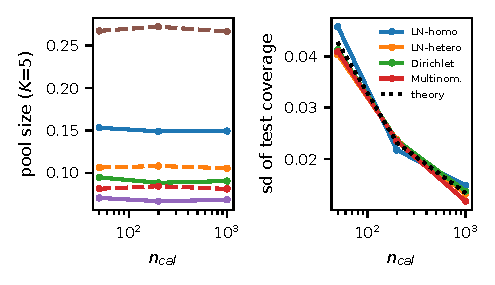
\includegraphics[width=0.5\textwidth]{fig_ncal.pdf}
\caption{Left: pool size vs.\ $n_{\rm cal}$ ($K=5$); right: standard deviation of test coverage across replicates for the $\ell_2$ score ($n_{\rm test}=1000$) with the theoretical value $\sqrt{\alpha(1-\alpha)(1/(n+2)+1/m)}$.}
\end{figure}

\begin{table}[h]
\caption{Paired relative size difference (first minus second, relative to second; $n_{\rm cal}=200$); $^*$: Holm-adjusted $p<0.05$ over 252 comparisons.}
\label{tab:paired}
\centering\small
\begin{tabular}{llrrrr}
\toprule
Comparison & $K$ & LN-homo & LN-hetero & Dirichlet & Multinom. \\
\midrule
Aitchison vs $\ell_2$ & 3 & -21\%* & -13\%* & +83\%* & +259\%* \\
 & 5 & -55\%* & -39\%* & +152\%* & +289\%* \\
 & 10 & -84\%* & -65\%* & +75\%* & +175\%* \\
\midrule
Hellinger vs $\ell_2$ & 3 & -17\%* & -15\%* & -12\%* & +14\%* \\
 & 5 & -41\%* & -34\%* & -22\%* & +26\%* \\
 & 10 & -69\%* & -58\%* & -40\%* & +20\%* \\
\midrule
Aitchison vs Hellinger & 3 & -5\%* & +2\% & +107\%* & +213\%* \\
 & 5 & -25\%* & -8\%* & +223\%* & +209\%* \\
 & 10 & -48\%* & -17\%* & +191\%* & +129\%* \\
\midrule
KL vs Hellinger & 3 & -1\%* & -2\%* & -2\%* & -17\%* \\
 & 5 & -0\% & -3\%* & -0\% & -30\%* \\
 & 10 & +1\% & -3\%* & +8\%* & -37\%* \\
\midrule
$\ell_2/\hat\sigma$ vs $\ell_2$ & 3 & -1\% & +1\% & -1\% & +1\% \\
 & 5 & +8\%* & +6\%* & +6\%* & +6\%* \\
 & 10 & +11\%* & +5\%* & +13\%* & +13\%* \\
\midrule
$\ell_2$-Mond. vs $\ell_2$ & 3 & +3\%* & +8\%* & +4\%* & +4\%* \\
 & 5 & +6\%* & +9\%* & +8\%* & +6\%* \\
 & 10 & +0\% & +6\%* & +10\%* & +10\%* \\
\midrule
Ait.-Mond. vs Aitchison & 3 & +4\%* & +6\%* & -13\%* & -17\%* \\
 & 5 & +6\%* & +7\%* & -12\%* & +2\%* \\
 & 10 & +8\%* & +5\% & -1\% & +4\%* \\
\bottomrule
\end{tabular}
\end{table}

\begin{table}[h]
\caption{Pool size for the full synthetic grid (bold: smallest).}
\label{tab:grid-size}
\centering\scriptsize
\setlength{\tabcolsep}{3pt}
\begin{tabular}{llrrrrrrrrrrr}
\toprule
DGP & $K$ & $n_{cal}$ & $\ell_2$ & TV & $\ell_\infty$ & Hellinger & KL & Aitchison & Mahal.-ilr & $\ell_2/\hat\sigma$ & $\ell_2$-Mond. & Ait.-Mond. \\
\midrule
LN-homo & 3 & 50 & 0.269 & 0.268 & 0.268 & 0.225 & 0.222 & \textbf{0.215} & 0.215 & 0.269 & 0.320 & 0.260 \\
LN-homo & 3 & 200 & 0.255 & 0.253 & 0.253 & 0.211 & 0.208 & \textbf{0.202} & 0.202 & 0.253 & 0.264 & 0.210 \\
LN-homo & 3 & 1000 & 0.255 & 0.252 & 0.252 & 0.211 & 0.209 & \textbf{0.203} & 0.203 & 0.253 & 0.255 & 0.205 \\
LN-homo & 5 & 50 & 0.153 & 0.133 & 0.185 & 0.095 & 0.094 & \textbf{0.070} & 0.071 & 0.165 & 0.215 & 0.105 \\
LN-homo & 5 & 200 & 0.149 & 0.128 & 0.179 & 0.088 & 0.088 & \textbf{0.067} & 0.067 & 0.160 & 0.158 & 0.071 \\
LN-homo & 5 & 1000 & 0.149 & 0.129 & 0.180 & 0.090 & 0.090 & \textbf{0.068} & 0.069 & 0.161 & 0.152 & 0.069 \\
LN-homo & 10 & 50 & 0.095 & 0.051 & 0.184 & 0.030 & 0.031 & \textbf{0.016} & 0.017 & 0.106 & 0.149 & 0.038 \\
LN-homo & 10 & 200 & 0.087 & 0.047 & 0.175 & 0.027 & 0.028 & \textbf{0.014} & 0.015 & 0.097 & 0.087 & 0.015 \\
LN-homo & 10 & 1000 & 0.083 & 0.046 & 0.168 & 0.026 & 0.027 & \textbf{0.013} & 0.014 & 0.093 & 0.079 & 0.014 \\
\midrule
LN-hetero & 3 & 50 & 0.210 & 0.208 & 0.208 & 0.181 & \textbf{0.179} & 0.189 & 0.189 & 0.213 & 0.295 & 0.270 \\
LN-hetero & 3 & 200 & 0.212 & 0.209 & 0.209 & 0.180 & \textbf{0.176} & 0.184 & 0.185 & 0.214 & 0.228 & 0.195 \\
LN-hetero & 3 & 1000 & 0.209 & 0.206 & 0.206 & 0.177 & \textbf{0.174} & 0.180 & 0.180 & 0.209 & 0.212 & 0.179 \\
LN-hetero & 5 & 50 & 0.148 & 0.128 & 0.176 & 0.100 & 0.097 & \textbf{0.093} & 0.093 & 0.159 & 0.250 & 0.169 \\
LN-hetero & 5 & 200 & 0.125 & 0.109 & 0.149 & 0.082 & 0.080 & \textbf{0.076} & 0.077 & 0.133 & 0.136 & 0.081 \\
LN-hetero & 5 & 1000 & 0.124 & 0.109 & 0.148 & 0.082 & 0.080 & 0.076 & 0.076 & 0.131 & 0.126 & \textbf{0.073} \\
LN-hetero & 10 & 50 & 0.088 & 0.053 & 0.158 & 0.037 & 0.036 & \textbf{0.029} & 0.031 & 0.094 & 0.170 & 0.067 \\
LN-hetero & 10 & 200 & 0.076 & 0.046 & 0.140 & 0.032 & 0.031 & \textbf{0.027} & 0.028 & 0.080 & 0.081 & 0.028 \\
LN-hetero & 10 & 1000 & 0.072 & 0.043 & 0.134 & 0.029 & 0.028 & 0.024 & 0.026 & 0.076 & 0.068 & \textbf{0.022} \\
\midrule
Dirichlet & 3 & 50 & 0.178 & 0.177 & 0.177 & 0.162 & \textbf{0.157} & 0.350 & 0.355 & 0.180 & 0.220 & 0.360 \\
Dirichlet & 3 & 200 & 0.175 & 0.175 & 0.175 & 0.155 & \textbf{0.152} & 0.321 & 0.323 & 0.174 & 0.181 & 0.278 \\
Dirichlet & 3 & 1000 & 0.172 & 0.172 & 0.172 & 0.154 & \textbf{0.151} & 0.325 & 0.328 & 0.172 & 0.173 & 0.271 \\
Dirichlet & 5 & 50 & 0.106 & 0.101 & 0.129 & \textbf{0.081} & 0.082 & 0.267 & 0.277 & 0.114 & 0.143 & 0.285 \\
Dirichlet & 5 & 200 & 0.108 & 0.103 & 0.129 & 0.084 & \textbf{0.084} & 0.272 & 0.280 & 0.115 & 0.116 & 0.241 \\
Dirichlet & 5 & 1000 & 0.105 & 0.101 & 0.126 & 0.081 & \textbf{0.081} & 0.267 & 0.276 & 0.111 & 0.108 & 0.226 \\
Dirichlet & 10 & 50 & 0.078 & 0.064 & 0.144 & \textbf{0.046} & 0.050 & 0.130 & 0.142 & 0.087 & 0.121 & 0.162 \\
Dirichlet & 10 & 200 & 0.076 & 0.062 & 0.144 & \textbf{0.046} & 0.050 & 0.134 & 0.146 & 0.086 & 0.084 & 0.132 \\
Dirichlet & 10 & 1000 & 0.072 & 0.059 & 0.136 & \textbf{0.044} & 0.047 & 0.130 & 0.141 & 0.082 & 0.075 & 0.123 \\
\midrule
Multinom. & 3 & 50 & 0.183 & 0.184 & 0.184 & 0.210 & \textbf{0.173} & 0.620 & 0.625 & 0.186 & 0.235 & 0.581 \\
Multinom. & 3 & 200 & 0.176 & 0.176 & 0.176 & 0.202 & \textbf{0.167} & 0.632 & 0.637 & 0.178 & 0.183 & 0.523 \\
Multinom. & 3 & 1000 & 0.177 & 0.177 & 0.177 & 0.201 & \textbf{0.168} & 0.631 & 0.636 & 0.178 & 0.178 & 0.495 \\
Multinom. & 5 & 50 & 0.115 & 0.112 & 0.134 & 0.141 & \textbf{0.099} & 0.426 & 0.435 & 0.122 & 0.159 & 0.468 \\
Multinom. & 5 & 200 & 0.114 & 0.111 & 0.132 & 0.144 & \textbf{0.101} & 0.443 & 0.452 & 0.120 & 0.121 & 0.451 \\
Multinom. & 5 & 1000 & 0.108 & 0.106 & 0.125 & 0.136 & \textbf{0.096} & 0.427 & 0.437 & 0.114 & 0.111 & 0.429 \\
Multinom. & 10 & 50 & 0.079 & 0.072 & 0.136 & 0.097 & \textbf{0.061} & 0.221 & 0.240 & 0.088 & 0.130 & 0.281 \\
Multinom. & 10 & 200 & 0.075 & 0.068 & 0.129 & 0.091 & \textbf{0.057} & 0.207 & 0.226 & 0.085 & 0.083 & 0.215 \\
Multinom. & 10 & 1000 & 0.074 & 0.067 & 0.128 & 0.089 & \textbf{0.056} & 0.206 & 0.225 & 0.083 & 0.076 & 0.208 \\
\bottomrule
\end{tabular}
\end{table}

\begin{table}[h]
\caption{Worst entropy-tercile coverage gap for the full synthetic grid.}
\label{tab:grid-gap}
\centering\scriptsize
\setlength{\tabcolsep}{3pt}
\begin{tabular}{llrrrrrrrrrrr}
\toprule
DGP & $K$ & $n_{cal}$ & $\ell_2$ & TV & $\ell_\infty$ & Hellinger & KL & Aitchison & Mahal.-ilr & $\ell_2/\hat\sigma$ & $\ell_2$-Mond. & Ait.-Mond. \\
\midrule
LN-homo & 3 & 50 & 0.059 & 0.064 & 0.064 & 0.057 & 0.054 & 0.009 & 0.008 & 0.023 & 0.026 & 0.031 \\
LN-homo & 3 & 200 & 0.058 & 0.063 & 0.063 & 0.058 & 0.055 & 0.003 & 0.003 & 0.022 & 0.008 & 0.009 \\
LN-homo & 3 & 1000 & 0.058 & 0.063 & 0.063 & 0.055 & 0.054 & 0.001 & 0.000 & 0.021 & 0.003 & 0.004 \\
LN-homo & 5 & 50 & 0.026 & 0.042 & 0.030 & 0.044 & 0.043 & 0.006 & 0.007 & 0.032 & 0.028 & 0.038 \\
LN-homo & 5 & 200 & 0.026 & 0.043 & 0.030 & 0.042 & 0.041 & 0.003 & 0.004 & 0.040 & 0.008 & 0.007 \\
LN-homo & 5 & 1000 & 0.025 & 0.042 & 0.029 & 0.042 & 0.040 & 0.003 & 0.003 & 0.039 & 0.003 & 0.002 \\
LN-homo & 10 & 50 & 0.034 & 0.020 & 0.031 & 0.028 & 0.028 & 0.013 & 0.016 & 0.051 & 0.028 & 0.029 \\
LN-homo & 10 & 200 & 0.036 & 0.019 & 0.034 & 0.025 & 0.025 & 0.020 & 0.018 & 0.054 & 0.010 & 0.010 \\
LN-homo & 10 & 1000 & 0.036 & 0.019 & 0.033 & 0.025 & 0.026 & 0.020 & 0.016 & 0.053 & 0.003 & 0.003 \\
\midrule
LN-hetero & 3 & 50 & 0.042 & 0.045 & 0.045 & 0.030 & 0.030 & 0.023 & 0.024 & 0.018 & 0.028 & 0.028 \\
LN-hetero & 3 & 200 & 0.045 & 0.048 & 0.048 & 0.033 & 0.034 & 0.019 & 0.019 & 0.017 & 0.010 & 0.009 \\
LN-hetero & 3 & 1000 & 0.046 & 0.049 & 0.049 & 0.034 & 0.035 & 0.017 & 0.017 & 0.015 & 0.004 & 0.003 \\
LN-hetero & 5 & 50 & 0.017 & 0.024 & 0.016 & 0.017 & 0.017 & 0.036 & 0.035 & 0.040 & 0.036 & 0.038 \\
LN-hetero & 5 & 200 & 0.020 & 0.024 & 0.022 & 0.016 & 0.016 & 0.030 & 0.031 & 0.034 & 0.007 & 0.010 \\
LN-hetero & 5 & 1000 & 0.020 & 0.021 & 0.021 & 0.014 & 0.014 & 0.034 & 0.033 & 0.035 & 0.002 & 0.002 \\
LN-hetero & 10 & 50 & 0.045 & 0.027 & 0.045 & 0.028 & 0.027 & 0.053 & 0.050 & 0.053 & 0.037 & 0.029 \\
LN-hetero & 10 & 200 & 0.044 & 0.022 & 0.045 & 0.024 & 0.024 & 0.051 & 0.048 & 0.050 & 0.010 & 0.008 \\
LN-hetero & 10 & 1000 & 0.045 & 0.022 & 0.045 & 0.023 & 0.022 & 0.054 & 0.052 & 0.052 & 0.002 & 0.002 \\
\midrule
Dirichlet & 3 & 50 & 0.055 & 0.058 & 0.058 & 0.027 & 0.025 & 0.104 & 0.102 & 0.017 & 0.033 & 0.033 \\
Dirichlet & 3 & 200 & 0.058 & 0.062 & 0.062 & 0.027 & 0.026 & 0.119 & 0.118 & 0.020 & 0.011 & 0.012 \\
Dirichlet & 3 & 1000 & 0.056 & 0.059 & 0.059 & 0.022 & 0.023 & 0.119 & 0.118 & 0.016 & 0.002 & 0.002 \\
Dirichlet & 5 & 50 & 0.039 & 0.055 & 0.037 & 0.029 & 0.024 & 0.086 & 0.087 & 0.025 & 0.024 & 0.030 \\
Dirichlet & 5 & 200 & 0.037 & 0.055 & 0.035 & 0.030 & 0.024 & 0.086 & 0.090 & 0.024 & 0.008 & 0.007 \\
Dirichlet & 5 & 1000 & 0.041 & 0.056 & 0.039 & 0.029 & 0.023 & 0.092 & 0.094 & 0.024 & 0.003 & 0.003 \\
Dirichlet & 10 & 50 & 0.024 & 0.063 & 0.013 & 0.046 & 0.034 & 0.071 & 0.069 & 0.031 & 0.033 & 0.033 \\
Dirichlet & 10 & 200 & 0.023 & 0.063 & 0.014 & 0.044 & 0.031 & 0.066 & 0.064 & 0.033 & 0.010 & 0.009 \\
Dirichlet & 10 & 1000 & 0.021 & 0.065 & 0.012 & 0.043 & 0.031 & 0.066 & 0.065 & 0.035 & 0.002 & 0.002 \\
\midrule
Multinom. & 3 & 50 & 0.064 & 0.066 & 0.066 & 0.027 & 0.020 & 0.067 & 0.067 & 0.022 & 0.035 & 0.032 \\
Multinom. & 3 & 200 & 0.060 & 0.063 & 0.063 & 0.023 & 0.014 & 0.067 & 0.067 & 0.015 & 0.007 & 0.010 \\
Multinom. & 3 & 1000 & 0.062 & 0.064 & 0.064 & 0.023 & 0.017 & 0.066 & 0.066 & 0.016 & 0.004 & 0.004 \\
Multinom. & 5 & 50 & 0.049 & 0.061 & 0.043 & 0.025 & 0.033 & 0.017 & 0.017 & 0.030 & 0.036 & 0.029 \\
Multinom. & 5 & 200 & 0.042 & 0.055 & 0.035 & 0.021 & 0.028 & 0.018 & 0.016 & 0.021 & 0.006 & 0.013 \\
Multinom. & 5 & 1000 & 0.045 & 0.058 & 0.037 & 0.024 & 0.031 & 0.015 & 0.013 & 0.023 & 0.002 & 0.002 \\
Multinom. & 10 & 50 & 0.024 & 0.065 & 0.011 & 0.062 & 0.050 & 0.037 & 0.034 & 0.034 & 0.031 & 0.035 \\
Multinom. & 10 & 200 & 0.023 & 0.063 & 0.011 & 0.061 & 0.051 & 0.033 & 0.031 & 0.033 & 0.009 & 0.007 \\
Multinom. & 10 & 1000 & 0.022 & 0.063 & 0.011 & 0.060 & 0.049 & 0.035 & 0.031 & 0.037 & 0.002 & 0.003 \\
\bottomrule
\end{tabular}
\end{table}

\section{Reproducibility Details}
\label{app:repro}
Code, results (CSV) and a step-by-step README are provided with the submission (\texttt{code/}, \texttt{results/}, \texttt{README.md}). Software: Python 3.11, NumPy 2.4.6, SciPy 1.17.1, pandas 3.0.6, Matplotlib 3.11.2, PyTorch 2.15.0 (CPU, inference only), PyArrow 26.0.1. Seeds: every synthetic run uses \texttt{np.random.SeedSequence([20261111, config\_id, replicate])} (CIFAR-10H: \texttt{[20261112, n\_cal, replicate]}; cross-conformal: \texttt{[20261113, config\_id, replicate]}; theory scripts: fixed seeds 1, 2, 3). Hardware: CPU only (shared 40-core machine under heavy load); wall-clock times observed with 30 worker processes: main grid 2030\,s, predictor-quality grid 1390\,s, $\varepsilon$ grid 270\,s, cross-conformal 430\,s, CIFAR-10H 140--300\,s, theory scripts about 10 min; figures and tables take under 5 minutes. No GPU was used.

\paragraph{Script to artefact map.}
\texttt{run\_theory.py} $\to$ Fig.~\ref{fig:theory}, Tables~\ref{tab:beta}, \ref{tab:k2gaps}, \ref{tab:zero}, Fig.~\ref{fig:zero}a; \texttt{run\_synth.py main} $\to$ Table~\ref{tab:main}, Figs.~\ref{fig:relsize}, \ref{fig:cond}, Tables~\ref{tab:validity}, \ref{tab:measure}, \ref{tab:paired}, \ref{tab:grid-size}, \ref{tab:grid-gap}; \texttt{run\_synth.py predq} $\to$ Table~\ref{tab:predq}; \texttt{run\_synth.py eps} $\to$ Fig.~\ref{fig:zero}b; \texttt{run\_cv.py} $\to$ Table~\ref{tab:cv}; \texttt{run\_cifar10h.py} $\to$ Table~\ref{tab:cifar}, Figs.~\ref{fig:zero}c, Tables~\ref{tab:cifar-ncal}, \ref{tab:cifar-eps}. Analysis: \texttt{analyze\_synth.py}, \texttt{analyze\_theory.py}, \texttt{analyze\_aux.py}.

\paragraph{Data and licences.} CIFAR-10 \citep{krizhevsky2009}: no licence stated on the dataset page (citation requested); we used the \texttt{uoft-cs/cifar10} parquet mirror on Hugging Face (downloaded first because the official server was slow), then downloaded the official tarball (md5 \texttt{c58f30108f718f92721af3b95e74349a}, as listed on the task page) and verified that the mirror's test images and labels are identical, in the same order, and that its training images are identical as a set (\texttt{code/verify\_cifar\_mirror.py}); the test order also matches CIFAR-10H (argmax of human proportions equals the test label for $99.2\%$ of images; a mismatched order would give about $10\%$). CIFAR-10H \citep{peterson2019cifar10h}: \texttt{cifar10h-probs.npy} from the authors' public repository; the repository states no licence in a LICENSE file (we checked); we use it for research only and do not redistribute it. The pretrained network is from \citet{chenyaofo2021cifar} (\texttt{cifar10\_resnet20}), loaded via \texttt{torch.hub}; it was trained on the CIFAR-10 training set only, so the 10000 test images are exchangeable and unseen.

\paragraph{Deviations and abandoned attempts.} (1) A first attempt to train a ResNet-9-style network on CPU was abandoned (the shared machine was too loaded; no results from it are used). (2) The ICML 2026 template was used (the NeurIPS 2026 style file was not available online at the time of writing; ICML 2026 is the latest edition whose official template we could obtain). (3) The CIFAR-10H experiment uses 100 replicates instead of 200 for compute reasons. (4) Uniform-measure size is not computed for $K=10$.

\paragraph{Literature access statement.} Literature consisted of the starter list and a small number of well-known papers whose bibliographic data (title, authors, arXiv identifier, year) were verified through the arXiv API or Crossref by identifier or exact title. No search was made for, and we did not encounter, the specific published paper the task excludes; nothing was read from any page that cites or discusses it.

\section{Checklist}
\begin{itemize}\setlength{\itemsep}{0pt}
\item \textbf{Claims match results and scope:} yes; scope and non-extrapolation conditions are in Sec.~\ref{sec:disc}.
\item \textbf{Limitations discussed:} yes (Sec.~\ref{sec:disc}); hypothesis H3 only partially supported and reported as such.
\item \textbf{Theory: assumptions and proofs:} Props.~\ref{prop:beta}--\ref{prop:zero}, assumptions stated, proofs in App.~\ref{app:proofs}, each checked numerically.
\item \textbf{Reproducibility:} code, seeds, commands, software versions, timings, script-to-table map (App.~\ref{app:repro}, README).
\item \textbf{Error bars / statistical significance:} 95\% CIs over replicates, paired differences with Holm correction, bootstrap CIs for group gaps.
\item \textbf{Data licences / provenance:} documented above; no personal data beyond the public CIFAR-10H aggregate proportions.
\item \textbf{Compute:} CPU only; no paid API.
\item \textbf{Ethics / impact:} see Impact Statement.
\end{itemize}


\end{document}
